\documentclass{standalone}
\usepackage{tikz}
\usetikzlibrary{patterns, positioning}
\usetikzlibrary{shapes.misc}
\usepackage[outline]{contour}
\contourlength{1.5pt} 
\usepackage[sfdefault]{ClearSans} %% option 'sfdefault' activates Clear Sans as the default text font
\usepackage[T1]{fontenc}

\begin{document}
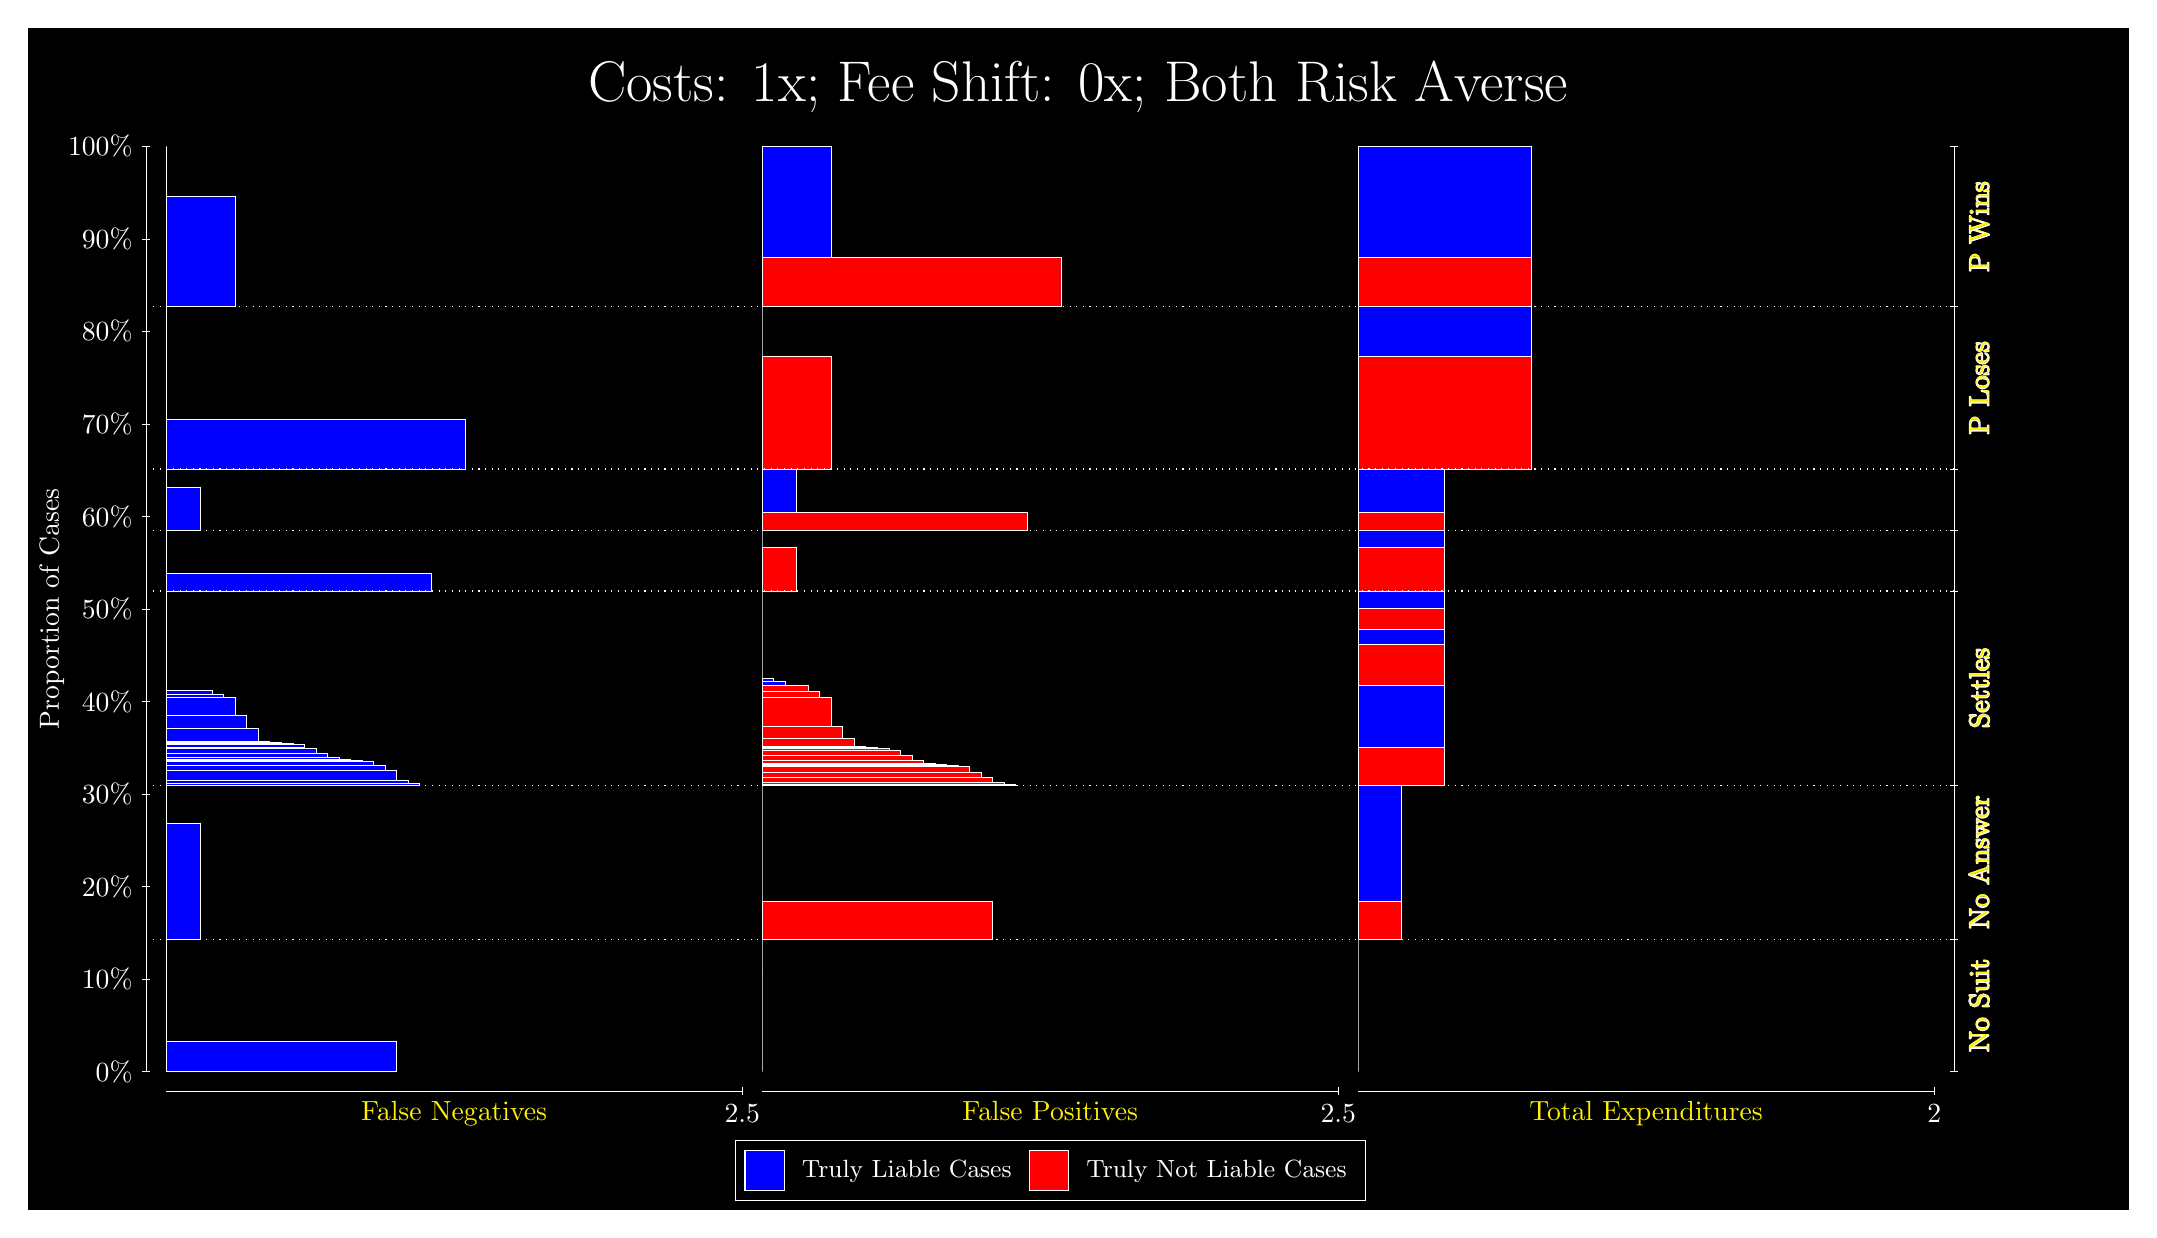
\begin{tikzpicture}
\draw[fill=black] (0,0) rectangle (26.667,15);
\draw[text=white] (0,13.5) rectangle (26.667,15) node[midway] {\huge Costs: 1x; Fee Shift: 0x; Both Risk Averse};
\draw[white, very thin] (1.5,1.75) -- (1.5,13.5);
\node[rotate=90, text=white, anchor=center] at (0.3, 7.625) {Proportion of Cases};
\draw[white, very thin] (1.45,1.75) -- (1.55,1.75);
\node[text=white, anchor=east] at (1.45, 1.75) {0\%};
\draw[white, very thin] (1.45,2.925) -- (1.55,2.925);
\node[text=white, anchor=east] at (1.45, 2.925) {10\%};
\draw[white, very thin] (1.45,4.1) -- (1.55,4.1);
\node[text=white, anchor=east] at (1.45, 4.1) {20\%};
\draw[white, very thin] (1.45,5.275) -- (1.55,5.275);
\node[text=white, anchor=east] at (1.45, 5.275) {30\%};
\draw[white, very thin] (1.45,6.45) -- (1.55,6.45);
\node[text=white, anchor=east] at (1.45, 6.45) {40\%};
\draw[white, very thin] (1.45,7.625) -- (1.55,7.625);
\node[text=white, anchor=east] at (1.45, 7.625) {50\%};
\draw[white, very thin] (1.45,8.8) -- (1.55,8.8);
\node[text=white, anchor=east] at (1.45, 8.8) {60\%};
\draw[white, very thin] (1.45,9.975) -- (1.55,9.975);
\node[text=white, anchor=east] at (1.45, 9.975) {70\%};
\draw[white, very thin] (1.45,11.15) -- (1.55,11.15);
\node[text=white, anchor=east] at (1.45, 11.15) {80\%};
\draw[white, very thin] (1.45,12.325) -- (1.55,12.325);
\node[text=white, anchor=east] at (1.45, 12.325) {90\%};
\draw[white, very thin] (1.45,13.5) -- (1.55,13.5);
\node[text=white, anchor=east] at (1.45, 13.5) {100\%};

\draw[white, very thin] (24.457,1.75) -- (24.457,13.5);
\draw[white, very thin] (24.407,1.75) -- (24.507,1.75);
\node[anchor=west] at (24.407, 1.75) {};
\draw[white, very thin] (24.407,3.4307) -- (24.507,3.4307);
\node[anchor=west] at (24.407, 3.4307) {};
\draw[white, very thin] (24.407,5.3879) -- (24.507,5.3879);
\node[anchor=west] at (24.407, 5.3879) {};
\draw[white, very thin] (24.407,7.8533) -- (24.507,7.8533);
\node[anchor=west] at (24.407, 7.8533) {};
\draw[white, very thin] (24.407,8.623) -- (24.507,8.623);
\node[anchor=west] at (24.407, 8.623) {};
\draw[white, very thin] (24.407,9.4014) -- (24.507,9.4014);
\node[anchor=west] at (24.407, 9.4014) {};
\draw[white, very thin] (24.407,11.463) -- (24.507,11.463);
\node[anchor=west] at (24.407, 11.463) {};
\draw[white, very thin] (24.407,13.5) -- (24.507,13.5);
\node[anchor=west] at (24.407, 13.5) {};

\draw[white, very thin, fill=blue] (1.75,1.75) rectangle (4.6775,2.139);
\draw[white, very thin, fill=red] (1.75,2.139) rectangle (1.75,3.4307);
\draw[white, very thin, fill=blue] (1.75,3.4307) rectangle (2.1891,4.9054);
\draw[white, very thin, fill=red] (1.75,4.9054) rectangle (1.75,5.3879);
\draw[white, very thin, fill=blue] (1.75,5.3879) rectangle (4.9703,5.4131);
\draw[white, very thin, fill=blue] (1.75,5.4131) rectangle (4.8239,5.4444);
\draw[white, very thin, fill=blue] (1.75,5.4444) rectangle (4.6775,5.5789);
\draw[white, very thin, fill=blue] (1.75,5.5789) rectangle (4.5312,5.638);
\draw[white, very thin, fill=blue] (1.75,5.638) rectangle (4.3848,5.6853);
\draw[white, very thin, fill=blue] (1.75,5.6853) rectangle (4.2384,5.7);
\draw[white, very thin, fill=blue] (1.75,5.7) rectangle (4.092,5.7068);
\draw[white, very thin, fill=blue] (1.75,5.7068) rectangle (4.092,5.7158);
\draw[white, very thin, fill=blue] (1.75,5.7158) rectangle (3.9457,5.7403);
\draw[white, very thin, fill=blue] (1.75,5.7403) rectangle (3.7993,5.7943);
\draw[white, very thin, fill=blue] (1.75,5.7943) rectangle (3.6529,5.8592);
\draw[white, very thin, fill=blue] (1.75,5.8592) rectangle (3.5065,5.8665);
\draw[white, very thin, fill=blue] (1.75,5.8665) rectangle (3.5065,5.9003);
\draw[white, very thin, fill=blue] (1.75,5.9003) rectangle (3.3602,5.9169);
\draw[white, very thin, fill=blue] (1.75,5.9169) rectangle (3.3602,5.918);
\draw[white, very thin, fill=blue] (1.75,5.918) rectangle (3.2138,5.9192);
\draw[white, very thin, fill=blue] (1.75,5.9192) rectangle (3.2138,5.931);
\draw[white, very thin, fill=blue] (1.75,5.931) rectangle (3.0674,5.9429);
\draw[white, very thin, fill=blue] (1.75,5.9429) rectangle (2.921,6.1149);
\draw[white, very thin, fill=blue] (1.75,6.1149) rectangle (2.7746,6.2798);
\draw[white, very thin, fill=blue] (1.75,6.2798) rectangle (2.6283,6.4986);
\draw[white, very thin, fill=blue] (1.75,6.4986) rectangle (2.4819,6.5393);
\draw[white, very thin, fill=blue] (1.75,6.5393) rectangle (2.3355,6.5897);
\draw[white, very thin, fill=red] (1.75,6.5897) rectangle (1.75,7.8533);
\draw[white, very thin, fill=blue] (1.75,7.8533) rectangle (5.1167,8.0731);
\draw[white, very thin, fill=red] (1.75,8.0731) rectangle (1.75,8.623);
\draw[white, very thin, fill=blue] (1.75,8.623) rectangle (2.1891,9.1715);
\draw[white, very thin, fill=red] (1.75,9.1715) rectangle (1.75,9.4014);
\draw[white, very thin, fill=blue] (1.75,9.4014) rectangle (5.5558,10.034);
\draw[white, very thin, fill=red] (1.75,10.034) rectangle (1.75,11.463);
\draw[white, very thin, fill=blue] (1.75,11.463) rectangle (2.6283,12.871);
\draw[white, very thin, fill=red] (1.75,12.871) rectangle (1.75,13.5);
\draw[white, very thin, fill=red] (9.3189,1.75) rectangle (9.3189,3.0416);
\draw[white, very thin, fill=blue] (9.3189,3.0416) rectangle (9.3189,3.4307);
\draw[white, very thin, fill=red] (9.3189,3.4307) rectangle (12.246,3.9131);
\draw[white, very thin, fill=blue] (9.3189,3.9131) rectangle (9.3189,5.3879);
\draw[white, very thin, fill=red] (9.3189,5.3879) rectangle (12.539,5.403);
\draw[white, very thin, fill=red] (9.3189,5.403) rectangle (12.393,5.4174);
\draw[white, very thin, fill=red] (9.3189,5.4174) rectangle (12.246,5.493);
\draw[white, very thin, fill=red] (9.3189,5.493) rectangle (12.1,5.5523);
\draw[white, very thin, fill=red] (9.3189,5.5523) rectangle (11.954,5.6245);
\draw[white, very thin, fill=red] (9.3189,5.6245) rectangle (11.807,5.6371);
\draw[white, very thin, fill=red] (9.3189,5.6371) rectangle (11.661,5.6495);
\draw[white, very thin, fill=red] (9.3189,5.6495) rectangle (11.661,5.6507);
\draw[white, very thin, fill=red] (9.3189,5.6507) rectangle (11.515,5.6518);
\draw[white, very thin, fill=red] (9.3189,5.6518) rectangle (11.515,5.6682);
\draw[white, very thin, fill=red] (9.3189,5.6682) rectangle (11.368,5.6982);
\draw[white, very thin, fill=red] (9.3189,5.6982) rectangle (11.368,5.7056);
\draw[white, very thin, fill=red] (9.3189,5.7056) rectangle (11.222,5.7687);
\draw[white, very thin, fill=red] (9.3189,5.7687) rectangle (11.075,5.8265);
\draw[white, very thin, fill=red] (9.3189,5.8265) rectangle (10.929,5.8506);
\draw[white, very thin, fill=red] (9.3189,5.8506) rectangle (10.783,5.8653);
\draw[white, very thin, fill=red] (9.3189,5.8653) rectangle (10.636,5.8672);
\draw[white, very thin, fill=red] (9.3189,5.8672) rectangle (10.636,5.8789);
\draw[white, very thin, fill=red] (9.3189,5.8789) rectangle (10.49,5.9777);
\draw[white, very thin, fill=red] (9.3189,5.9777) rectangle (10.344,6.1325);
\draw[white, very thin, fill=red] (9.3189,6.1325) rectangle (10.197,6.5037);
\draw[white, very thin, fill=red] (9.3189,6.5037) rectangle (10.051,6.5797);
\draw[white, very thin, fill=red] (9.3189,6.5797) rectangle (9.9044,6.6515);
\draw[white, very thin, fill=blue] (9.3189,6.6515) rectangle (9.6116,6.7019);
\draw[white, very thin, fill=blue] (9.3189,6.7019) rectangle (9.4652,6.7425);
\draw[white, very thin, fill=blue] (9.3189,6.7425) rectangle (9.3189,7.8533);
\draw[white, very thin, fill=red] (9.3189,7.8533) rectangle (9.758,8.4032);
\draw[white, very thin, fill=blue] (9.3189,8.4032) rectangle (9.3189,8.623);
\draw[white, very thin, fill=red] (9.3189,8.623) rectangle (12.686,8.8529);
\draw[white, very thin, fill=blue] (9.3189,8.8529) rectangle (9.758,9.4014);
\draw[white, very thin, fill=red] (9.3189,9.4014) rectangle (10.197,10.83);
\draw[white, very thin, fill=blue] (9.3189,10.83) rectangle (9.3189,11.463);
\draw[white, very thin, fill=red] (9.3189,11.463) rectangle (13.125,12.092);
\draw[white, very thin, fill=blue] (9.3189,12.092) rectangle (10.197,13.5);
\draw[white, very thin, fill=red] (16.888,1.75) rectangle (16.888,3.0416);
\draw[white, very thin, fill=blue] (16.888,3.0416) rectangle (16.888,3.4307);
\draw[white, very thin, fill=red] (16.888,3.4307) rectangle (17.437,3.9131);
\draw[white, very thin, fill=blue] (16.888,3.9131) rectangle (17.437,5.3879);
\draw[white, very thin, fill=red] (16.888,5.3879) rectangle (17.986,5.8698);
\draw[white, very thin, fill=blue] (16.888,5.8698) rectangle (17.986,6.6549);
\draw[white, very thin, fill=red] (16.888,6.6549) rectangle (17.986,7.1758);
\draw[white, very thin, fill=blue] (16.888,7.1758) rectangle (17.986,7.3688);
\draw[white, very thin, fill=red] (16.888,7.3688) rectangle (17.986,7.6296);
\draw[white, very thin, fill=blue] (16.888,7.6296) rectangle (17.986,7.8533);
\draw[white, very thin, fill=red] (16.888,7.8533) rectangle (17.986,8.4032);
\draw[white, very thin, fill=blue] (16.888,8.4032) rectangle (17.986,8.623);
\draw[white, very thin, fill=red] (16.888,8.623) rectangle (17.986,8.8529);
\draw[white, very thin, fill=blue] (16.888,8.8529) rectangle (17.986,9.4014);
\draw[white, very thin, fill=red] (16.888,9.4014) rectangle (19.083,10.83);
\draw[white, very thin, fill=blue] (16.888,10.83) rectangle (19.083,11.463);
\draw[white, very thin, fill=red] (16.888,11.463) rectangle (19.083,12.092);
\draw[white, very thin, fill=blue] (16.888,12.092) rectangle (19.083,13.5);
\draw[white, dotted] (1.5,3.4307) -- (24.457,3.4307);
\draw[white, dotted] (1.5,5.3879) -- (24.457,5.3879);
\draw[white, dotted] (1.5,7.8533) -- (24.457,7.8533);
\draw[white, dotted] (1.5,8.623) -- (24.457,8.623);
\draw[white, dotted] (1.5,9.4014) -- (24.457,9.4014);
\draw[white, dotted] (1.5,11.463) -- (24.457,11.463);
\draw[white, very thin] (1.75,1.5) -- (9.0689,1.5);
\node[text=yellow, anchor=north] at (5.4094, 1.5) {False Negatives};
\draw[white, very thin] (9.0689,1.45) -- (9.0689,1.55);
\node[text=white, anchor=north] at (9.0689, 1.45) {2.5};

\draw[white, very thin] (9.3189,1.5) -- (16.638,1.5);
\node[text=yellow, anchor=north] at (12.978, 1.5) {False Positives};
\draw[white, very thin] (16.638,1.45) -- (16.638,1.55);
\node[text=white, anchor=north] at (16.638, 1.45) {2.5};

\draw[white, very thin] (16.888,1.5) -- (24.207,1.5);
\node[text=yellow, anchor=north] at (20.547, 1.5) {Total Expenditures};
\draw[white, very thin] (24.207,1.45) -- (24.207,1.55);
\node[text=white, anchor=north] at (24.207, 1.45) {2};

\node[text=yellow, centered, rotate=90] at (24.777, 2.5903) {\contour{white}{No Suit}};
\node[text=yellow, centered, rotate=90] at (24.777, 4.4093) {\contour{white}{No Answer}};
\node[text=yellow, centered, rotate=90] at (24.777, 6.6206) {\contour{white}{Settles}};


\node[text=yellow, centered, rotate=90] at (24.777, 10.432) {\contour{white}{P Loses}};
\node[text=yellow, centered, rotate=90] at (24.777, 12.481) {\contour{white}{P Wins}};

\draw (12.978300999999998,1.5) node[draw=none] (baseCoordinate) {};
\begin{scope}[align=center]
        \matrix[scale=0.5, draw=white, below=0.5cm of baseCoordinate, nodes={draw}, column sep=0.1cm]{
            \node[rectangle, draw, minimum width=0.5cm, minimum height=0.5cm, fill=blue] {}; &
            \node[draw=none, font=\small, text=white] (B) {Truly Liable Cases}; &
            \node[rectangle, draw, minimum width=0.5cm, minimum height=0.5cm, fill=red] {}; &
            \node[draw=none, font=\small, text=white] (B) {Truly Not Liable Cases}; \\
            };
\end{scope}

\end{tikzpicture}
\end{document}